\section{Modeling, extension, and cross-solver comparison}
\label{chapter:04}

% block-id: auto.04.heading1
\hypertarget{auto.04.heading1}{}
\subsection{Wolfram calibration and model extension}

% block-id: auto.04.p1
\hypertarget{auto.04.p1}{}
The archived rc.2 Wolfram case records MCP initialization, tool discovery, and actual calls, connecting analytical calculation, testing, graphics, and Notebook persistence. At 200 kHz, the round-wire reference gives Rac=\metric{q1_rac} mΩ/m and a loss of \metric{q1_loss} W/m. Independent complex-current and Joule-power integrals check normalization and the RMS convention. The analytical reference and native Notebook tooling are supported by the mathematical definitions and the AgentTools interface, respectively. \cite{BESSEL,AGENTTOOLS}

% block-id: auto.04.figure
\hypertarget{auto.04.figure}{}
\begin{figure*}[!htbp]
\centering
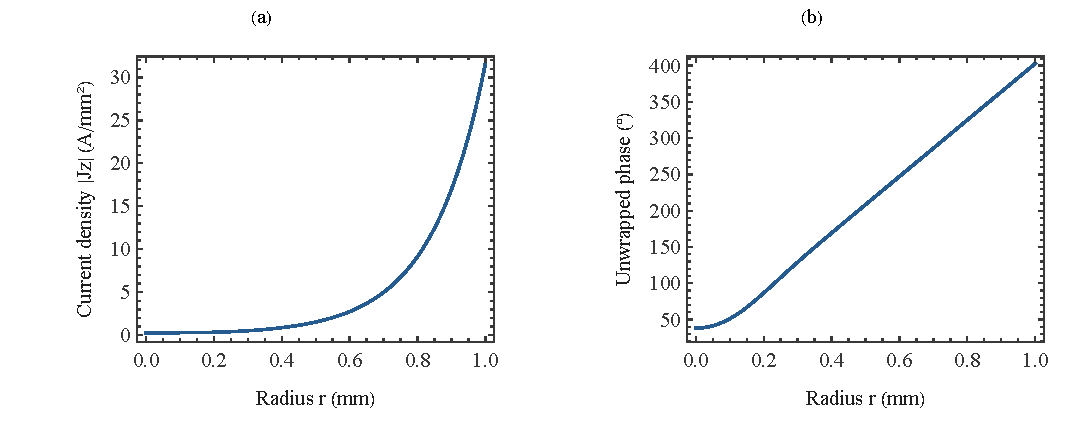
\includegraphics[width=\linewidth,height=.72\textheight,keepaspectratio]{../../assets/en/q1_profile.pdf}
\caption{Round-wire radial current magnitude and phase. The copper conductor has diameter 2 mm and carries 20 A RMS at 200 kHz. (a) RMS magnitude; (b) continuously displayed phase. Phase is displayed with a continuous radial lift, while magnitude retains RMS normalization. Radial samples come from preserved Bessel analytical data.}
\label{fig:q1_profile}
\end{figure*}

% block-id: auto.04.p2
\hypertarget{auto.04.p2}{}
The frequency-extension case expands the single-frequency analytical implementation into a frequency study. It retains the source difference, parameters, and new results and checks integrals, the low-frequency limit, and regression against the original case. This example demonstrates how agent edits can enter the research workflow through deterministic checks. Its acceptance covers the analytical implementation and tested frequency conditions; adding material dispersion or thermal coupling would require corresponding physical checks.

% block-id: auto.04.heading2
\hypertarget{auto.04.heading2}{}
\subsection{Maxwell construction, solution, and comparison}

% block-id: auto.04.p3
\hypertarget{auto.04.p3}{}
The Ansys case connects MCP to a runner-owned session and completes material assignment, excitation, solution, and result retrieval for a small seven-strand Maxwell model. The rc2\_maxwell\_mcp\_verified\_01 run and its linked recovery pass checks within the port-and-power scope; protocol probes retain their own protocol status. Task cancellation and recovery under a new identifier have separate records, allowing the relationship between task identity and actual AEDT execution to be inspected.

% block-id: auto.04.p4
\hypertarget{auto.04.p4}{}
The Wolfram–Maxwell comparison uses seven straight insulated strands, common terminal voltage, a total-current constraint, and a controlled copper return. Alignment checks cover strand count, polygonal cross-section, strand diameter, return inner and outer radii, exterior-domain radius, axial depth, frequency, and total current. The retained comparison gives a relative L2 difference of 0.0106814\% in complex strand currents and a relative bundle Rac difference of 0.00132823\%; the corresponding resistances are 318.290316 and 318.294544 mΩ per axial metre.

% block-id: auto.04.p5
\hypertarget{auto.04.p5}{}
These values describe agreement between implementations for this case. The implementations use independent meshes and interpolation orders, the conductor cross-sections are 42-sided polygons, and return segmentation may differ. Maxwell uses one adaptive pass, with spatial and boundary convergence still to be established. The case's copper area is below the Q2 requirement. The comparison therefore checks the common-port implementation across solvers; further accuracy estimation requires varying meshes and boundaries and analyzing the resulting changes.
